\subsection{Prototypes}\label{sec:sprint2:prototypes}

At the end of first sprint, the existing features of \launcher were polished and the project would only need to be kept updated with the implementation of the database. \vagner{Verify that this is indeed what actually happened}
However, the review meeting of sprint one determined that it was desired for launcher to possibly have additional features:

\begin{itemize}
\item Selection of profiles might be desired to be selectable elsewhere in \launcher without starting an application.
\item Settings for different applications could be set from an activity accessed from \launcher.
\item Specification of which applications different users can access could likewise be set from and accessed from \launcher.
\end{itemize}

It was decided to have a brainstorm to gather ideas regarding these features, create prototypes of the best ones\footnote{The prototypes regarded as being the best, were deemed so by the project group.} and present these to the customers for feedback.

The prototypes created were \textbf{low fidelity, horizontal} prototypes, as described in \citet[p. 184-195]{debBook}, made partly with screenshots of existing functionality and partly with the modelling tool Gliffy (\citet{gliffy}).
The purpose was to convey several different ways of including the above features, while not spending too much time creating them.

\subsubsection{Profile Selection}

At the end of sprint one, the profile selection would only appear when launching an application, as illustrated by the state chart diagram in \Cref{fig:statechartProfileSelectorInitial}.
\insertfigure{width=\textwidth}{statechartProfileSelectorInitial}{State chart diagram for the original process of choosing a profile.}{fig:statechartProfileSelectorInitial}
Two alternatives where suggested:
\begin{itemize}
\item Selection of a different profile from within \launcher.
This would work by pressing the profile picture, giving a list of profiles to choose from.
Being relevant only for a guardian, the profiles selectable should only be the guardian itself and the child related to him or her.

\item Selection of a different profile from within each individual application.
While this solution does not require any modification of \launcher, it was a favourable option.
Each application would then have its own profile selection button to initiate the activities
\end{itemize}

Common for both alternatives was to display the currently selected profile in the top of the pane.
Illustrations can be seen on \Cref{fig:profileselectionlauncherdropdown,fig:profileselectionapppopup} respectively. For an explanation of the suggested process of choosing a profile see the state chart diagram in \Cref{fig:statechartProfileSelectorBubble}.

\begin{figure}[h] % Billeder af profile selector
\centering
    \begin{subfigure}[t]{.48\textwidth}
    \centering
    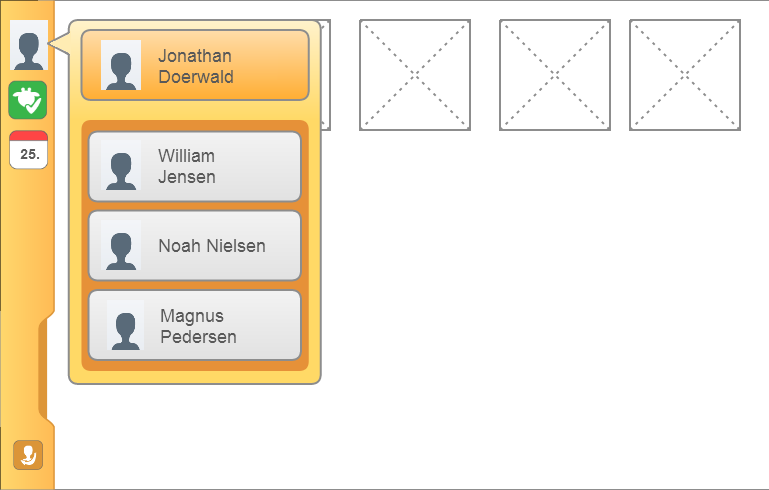
\includegraphics[width=\textwidth]{sprint2/profileselectionhomescreen-dropdown}
    \caption{The dropdown profile selection option. This would appear when tapping ones profile picture as a guardian.}
    \label{fig:profileselectionlauncherdropdown}
    \end{subfigure}
    \hfill
    \begin{subfigure}[t]{.48\textwidth}
    \centering
    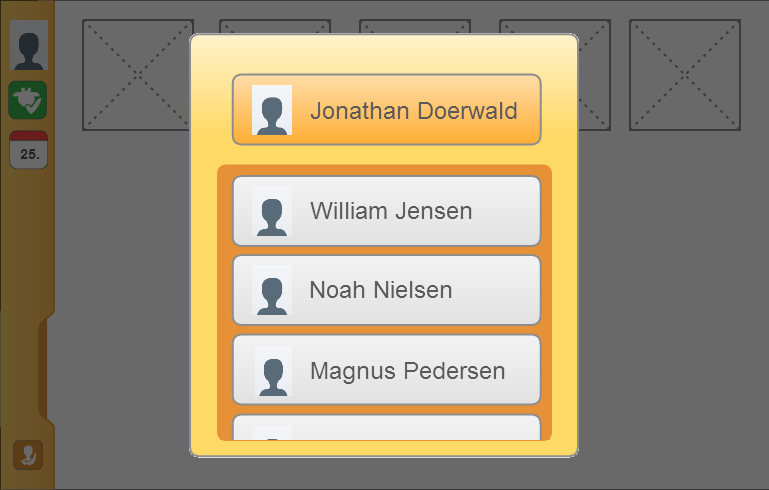
\includegraphics[width=\textwidth]{sprint2/profileselection-dialog-finish}
    \caption{The profile selection pop up. These would only appear while pressing the appropriate button while inside an application.}
    \label{fig:profileselectionapppopup}
    \end{subfigure}\\
    \begin{center}
    \begin{subfigure}[t]{1\textwidth}
    \includegraphics[width=\textwidth]{figures/statechartProfileSelectorBubble.tikz}
    \caption{State chart diagram for the suggested alternative process of choosing a profile.}
    \label{fig:statechartProfileSelectorBubble}
    \end{subfigure}
    \end{center}

\caption{Suggestions for the new profile selector.}
\label{fig:drawerstates}
\end{figure}

\subsubsection{Settings}

At the end of first sprint, settings for different applications where handled inside those applications exclusively.
The idea of centralizing the settings for the different applications was formed both to streamline data for the database, but also to grant the user a better overview over the settings shared by applications.

Again, two alternatives were presented:
\begin{itemize}
\item A settings activity, accessible from \launcher only.
This activity would contain settings for all applications enabled for the selected user, as well as selecting which applications should be enabled for that profile.
This would also include the native Android settings.
\item Letting each application have a settings button.
This would preserve the current setup.
\end{itemize}

The first option is the most encompassing one, containing functionality for both manipulate settings for other applications and decide which applications can be used with different users.
It was furthermore discussed to add functionality, allowing the user to add applications from Google Play to \launcher.
The settings part of the settings activity can be seen in \Cref{fig:settingsprototype}, while the application management part can be seen in \Cref{fig:appsmanagement}.

The second option is more centred on making the settings screen streamlined across applications and would thus be a operative project with the GUI project group.
An example of settings for \launcher can be seen in \Cref{fig:appsettingsprototype}.

\begin{figure}[h] % Billeder af draweren i �ben og lukket tilstand
\centering
    \begin{subfigure}[t]{.48\textwidth}
    \centering
    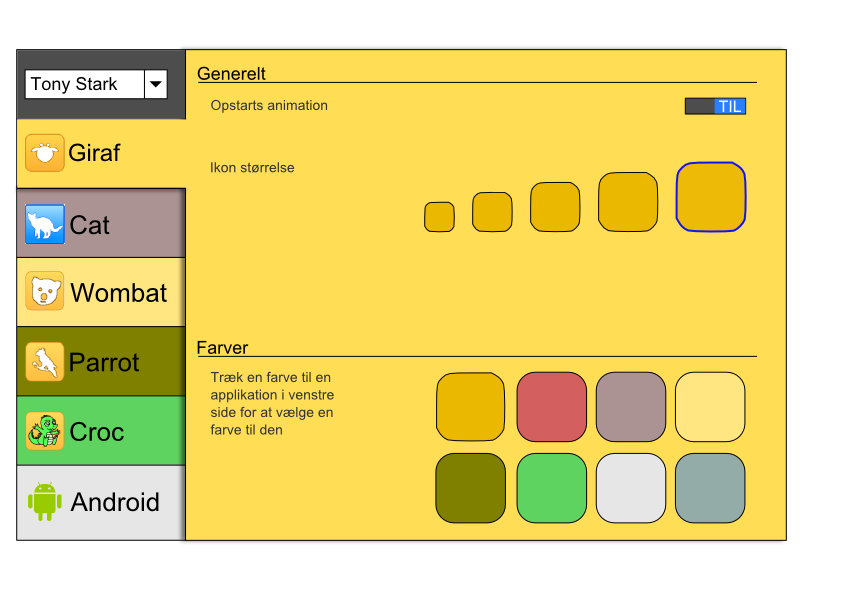
\includegraphics[width=\textwidth]{sprint2/settings}
    \caption{The settings manipulation part of the settings application. in this example, settings for \launcher can be seen. The current profile being edited can be seen in the top left corner.}
    \label{fig:settingsprototype}
    \end{subfigure}
    \hfill
    \begin{subfigure}[t]{.48\textwidth}
    \centering
    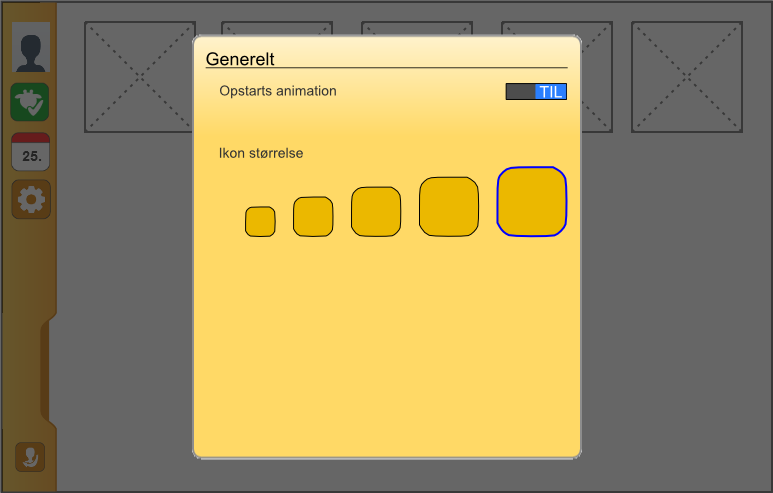
\includegraphics[width=\textwidth]{sprint2/settings-dialog}
    \caption{The settings for a single application. In this example, the settings for \launcher can be seen.}
    \label{fig:appsettingsprototype}
    \end{subfigure}\\
    \begin{subfigure}[t]{.48\textwidth}
    \centering
    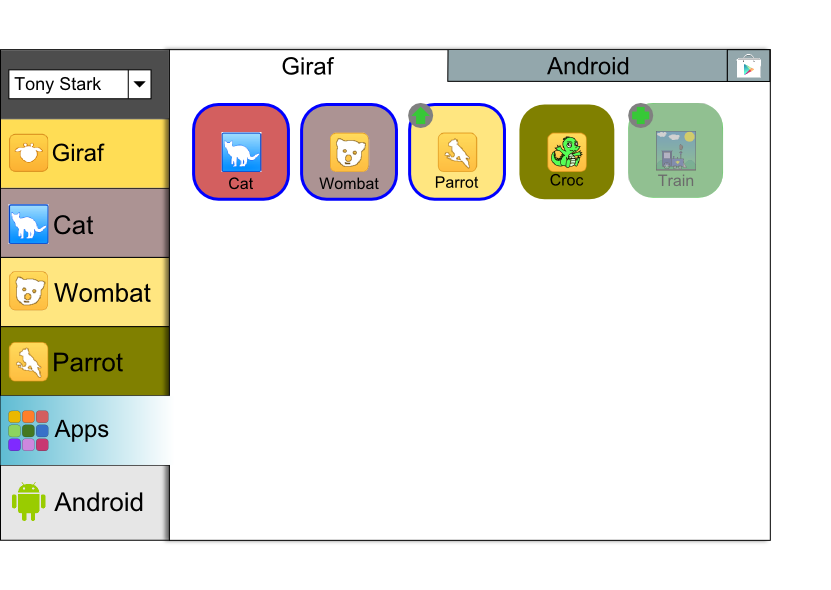
\includegraphics[width=\textwidth]{sprint2/apps-colorexperiment}
    \caption{The application management part of the settings application. \giraf or Android (Google Play) applications can be chosen in the pane in the top. The current profile being edited can be seen in the top left corner.}
    \label{fig:appsmanagement}
    \end{subfigure}
\caption{Suggestions for settings and application management.}
\label{fig:drawerstates}
\end{figure}

\subsubsection{Profile Info}
\frederik{Maaske vi skal undlade denne section, kunderne var ikke vilde med det.}
The group had an idea of displaying information about the user currently logged in in the drawer section of \launcher.
This is a relatively small feature that would be trivial to implement.
An example can be seen in \Cref{fig:profileinfo}.

\insertfigure{width=0.48\textwidth}{sprint2/profil-info}{An example of information about a user seen in the drawer.}{fig:profileinfo}